%!TEX TS-program = xelatex
\documentclass{beamer}

\usepackage{amsmath,amssymb}
\usepackage{graphicx}
\usepackage{mcode}
\usepackage{colortbl}
\usepackage{times}
\usepackage{pstcol,pst-node,pst-plot}
\usepackage{pstricks,pst-plot}
\usepackage{txfonts}
\usepackage{hyperref}
\hypersetup{
    colorlinks,
    citecolor=black,
    filecolor=black,
    linkcolor=black,
    urlcolor=black
}
\usepackage{authblk}

\title{Experiment in the form of slides}

\begin{document}

\maketitle

\begin{frame}{Introduction}
	\begin{scriptsize}
	\begin{itemize}
		\item Thank you for your participation in this survey. 
		\item Please take as much time as you need to answer the questions.
		Questions only require you to check a box or select a graphic by clicking.
		All your answers to the questions are strictly anonymous. No one will
		contact you after the survey, and no sales solicitation is involved.
		Your answers will be used for research purposes only.
		\item Please DO NOT USE the ``Back'' and ``Forward'' buttons in your
		browser. Please use the buttons at the bottom of each screen.
		\item If you would like to pause the survey to return to it later, simply close the window and click on the original link in the invitation. It will return you to the last point of entry in the survey.
		\item Please click on `` $>>$ '' to start the survey.	
	\end{itemize}
	\end{scriptsize}
\end{frame}

\begin{frame}{Male Stars}
Which movie star would you choose to have lunch with?

\begin{itemize}
	\item Tom Hanks
	\item Kevin Spacey
	\item Morgan Freeman
	\item Leonardo DiCaprio
	\item Christian Bale
\end{itemize}
\end{frame}

\begin{frame}{Female Stars}
Which movie star would you choose to have lunch with?

\begin{itemize}
	\item Meryl Streep
	\item Jody Foster
	\item Kathy Bates
	\item Amy Adams
	\item Julianne Moore
\end{itemize}
\end{frame}

\begin{frame}{Films}
Judging from the following descriptions of films, which one of the films would you choose to see?

\begin{itemize}
	\item Two imprisoned men bond over a number of years, finding solace and
eventual redemption through acts of common decency. \\
	\item Mathilda, a 12-year-old girl, is reluctantly taken in by L\'eon, a
professional assassin, after her family is murdered. L\'eon and Mathilda
form an unusual relationship, as she becomes his prot\'eg\'e and learns the
assassin's trade. \\
	\item The lives of two mob hit men, a boxer, a gangster's wife, and a pair
of diner bandits intertwine in four tales of violence and redemption. \\
	\item A sexually frustrated suburban father has a mid-life crisis after
becoming infatuated with his daughter's best friend. \\
	\item Identical twins, separated at birth and each raised by one of their
biological parents, discover each other for the first time at summer camp
and make a plan to bring their wayward parents back together.
\end{itemize}
\end{frame}

\begin{frame}{Star pairs}
Knowing only who is starring, which one of these new films would you choose to see?

\begin{itemize}
	\item Tom Hanks and Scarlett Johansson
	\item Scarlett Johansson and Brad Pitt
	\item Tom Hanks and Brad Pitt
	\item Scarlett Johansson and Angelina Jolie
	\item Tom Hanks and Angelina Jolie
\end{itemize}
\end{frame}

\begin{frame}{Pizzas}
Which one of the following pizzas would you choose?

\begin{itemize}
	\item Mozzarella, tomato sauce, basil
	\item Pepperoni, mushrooms, green pepper, mozzarella, tomato sauce
	\item Red onion, tomato sauce, feta, mozzarella, olive oil, Greek spices,
tomato sauce
	\item Bacon, white onion, mozzarella, parmesan, fresh cream, tomato sauce,
ground pepper
	\item Mushrooms, green pepper, mozzarella, tomato sauce
\end{itemize}
\end{frame}

\begin{frame}{Juices}
Which one of the following fresh juices would you choose?

\begin{itemize}
	\item Mango
	\item Orange
	\item Apple
	\item Grapefruit
	\item Pineapple
\end{itemize}
\end{frame}

\begin{frame}{Colours}
Which one of the following colours do you like best?

\begin{itemize}
	\item Red
	\item Purple
	\item Pink
	\item Blue
	\item Green
\end{itemize}
\end{frame}

\begin{frame}{Color combinations}
Which one of these colour combinations do you like best?

\begin{itemize}
	\item Black and red
	\item Black and purple
	\item Black and blue
	\item Blue and red
	\item Blue and purple
\end{itemize}
\end{frame}

\begin{frame}{Events}
Which one of the following events do you think is most likely to happen in the next twenty years?

\begin{itemize}
	\item Scotland becomes an independent country.
	\item Either Catalonia or Quebec become independent countries.
	\item Catalonia becomes an independent country.
	\item Scotland and Quebec become independent countries.
	\item Either Scotland or Quebec become independent countries.
\end{itemize}
\end{frame}

\begin{frame}{Radio formats}
Suppose you were on a two hour road trip and you have a choice among radio stations with the following formats.
Which one would you choose?

\begin{itemize}
	\item News
	\item Hot Adult Contemporary, or Hot AC
	(A variety of classic and contemporary mainstream music geared towards adults.)
	\item Classic Hits (Rock and pop, roughly 1964-1989)
	\item Country Music
	\item Adult Contemporary, or AC (Adult-oriented pop/rock with no hard rock.)
\end{itemize}
\end{frame}

\begin{frame}{Musical artists}
Which one of the following musical artists do you like the best?

\begin{itemize}
	\item The Beatles
	\item Elvis Presley
	\item Michael Jackson
	\item Madonna
	\item Elton John
\end{itemize}
\end{frame}

\begin{frame}{Aboriginal art}
Which one of the following examples of Australian aboriginal art do you like the best?

\vspace{0.5cm}
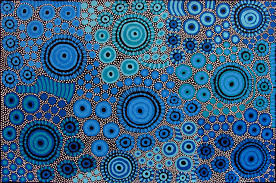
\includegraphics[width=2cm]{Aboriginal_art1.jpg}
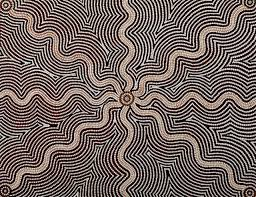
\includegraphics[width=2cm]{Aboriginal_art2.jpg}

\includegraphics[width=2cm]{Aboriginal_art3.jpg}

\includegraphics[width=2cm]{Aboriginal_art4.jpg}
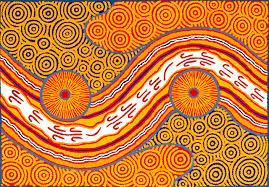
\includegraphics[width=2cm]{Aboriginal_art5.jpg}
\end{frame}

\begin{frame}{Impressionist art}
Which one of the following examples of Impressionist art do you like the best?

\vspace{0.5cm}
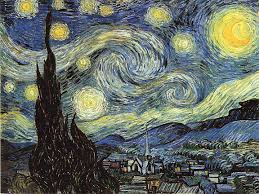
\includegraphics[width=2cm]{Impressionist_art1.jpg}
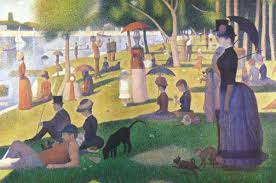
\includegraphics[width=2cm]{Impressionist_art2.jpg}
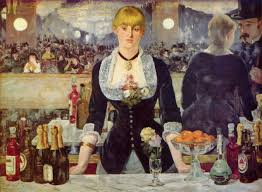
\includegraphics[width=2cm]{Impressionist_art3.jpg}
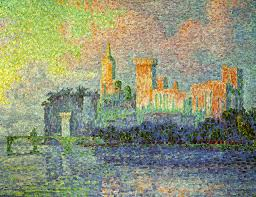
\includegraphics[width=2cm]{Impressionist_art4.jpg}
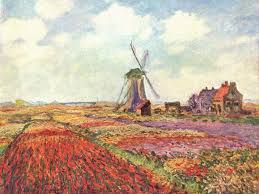
\includegraphics[width=2cm]{Impressionist_art5.jpg}
\end{frame}

\begin{frame}{Sentences}
Which one of the following sentences do you find the most grammatically acceptable?

\begin{itemize}
	\item Who did Bill buy the car to please?
	\item This is a book which reading would be fun.
	\item Where did Bill buy the car to drive?
	\item Which man do you wonder when to meet?
	\item With which pen do you wonder what to write?
\end{itemize}
\end{frame}

\begin{frame}{Travel}
Which one of the following travel destinations would you most like to visit?

\begin{enumerate}
\item Marrakech, Morocco
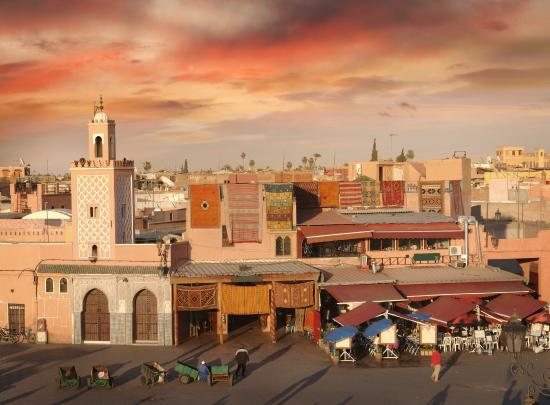
\includegraphics[height=1.4cm]{Travel1.jpg}

\item Istanbul, Turkey
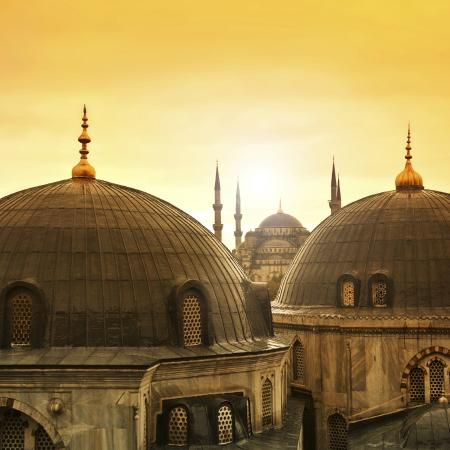
\includegraphics[height=1.4cm]{Travel2.jpg}

\item Hanoi, Vietnam
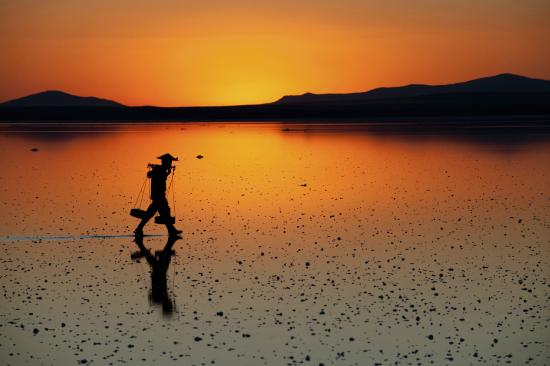
\includegraphics[height=1.4cm]{Travel3.jpg}

\item Siem Reap, Cambodia
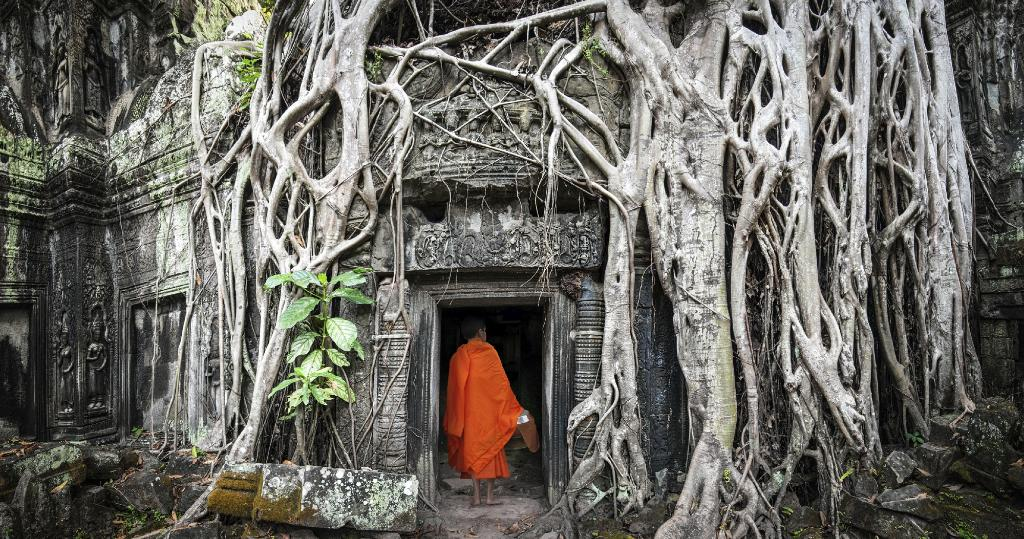
\includegraphics[height=1.4cm]{Travel4.jpg}

\item Praque, Czech Republic
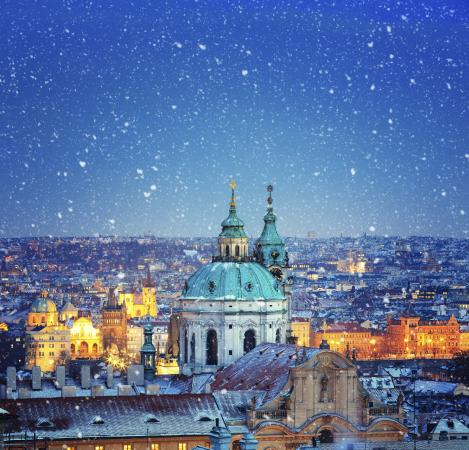
\includegraphics[height=1.4cm]{Travel5.jpg}
\end{enumerate}	
\end{frame}

\begin{frame}{Marijuana}
Which one of the following marijuana policies would you choose?

\begin{itemize}
	\item Possession by, and sales to adults are both legal; sales to minors are illegal.
	\item Possession by, and sales to adults are both illegal but neither is a criminal offense; sales to minors are a criminal offense.
	\item Possession is illegal but not criminal; all sales are a criminal offense.
	\item Possession and sales are criminal offenses, with a small number of medical exceptions.
	\item Possession and sales are criminal offenses, without exception.
\end{itemize}
\end{frame}

\begin{frame}{Latitude}
Which one of the following cities do you think is furthest north?

\begin{itemize}
	\item Warsaw, Poland
	\item London, United Kingdom
	\item Vancouver, Canada
	\item Paris, France
	\item Seattle, United States
\end{itemize}
\end{frame}

\begin{frame}{Scatterplots}
Which one of the following boxes do you think has the greatest number of points?

\vspace{0.5cm}
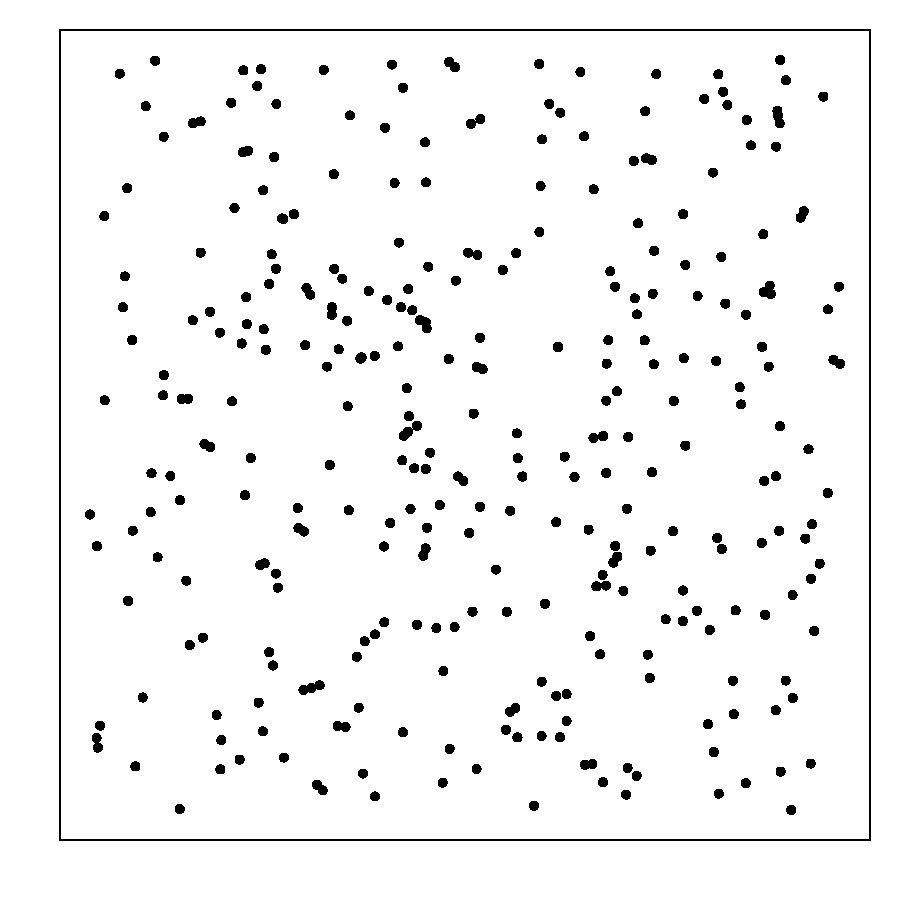
\includegraphics[height=2cm]{Scatterplots1.pdf}
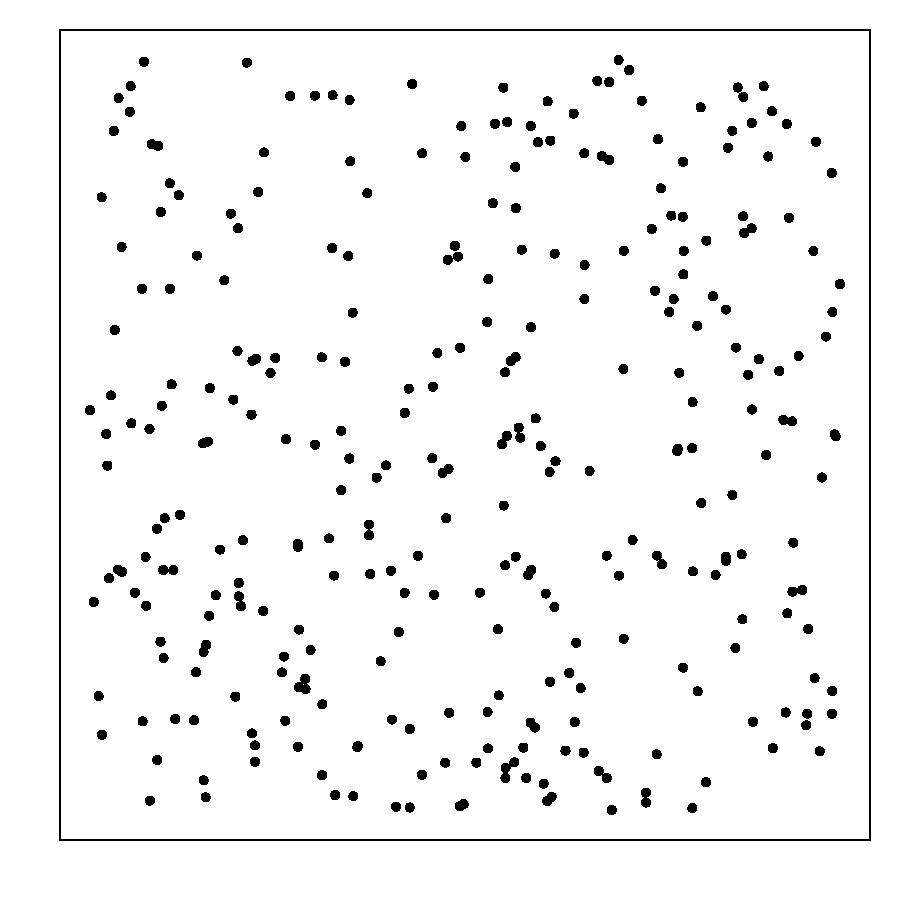
\includegraphics[height=2cm]{Scatterplots2.pdf}
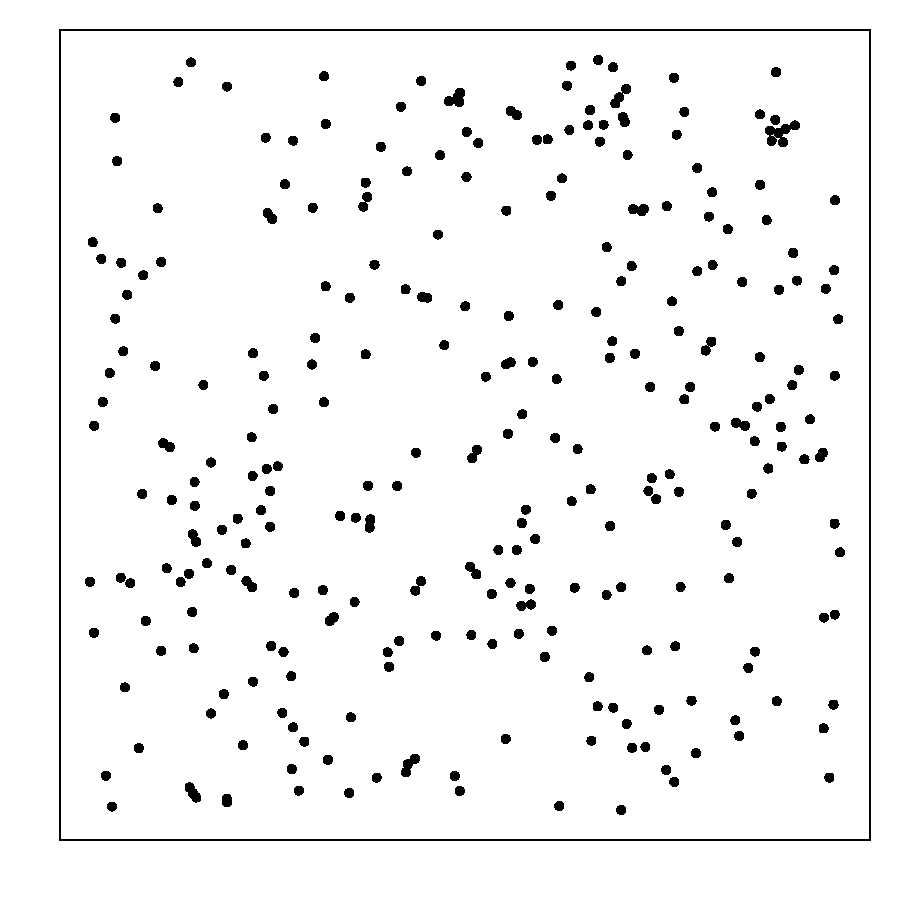
\includegraphics[height=2cm]{Scatterplots3.pdf}
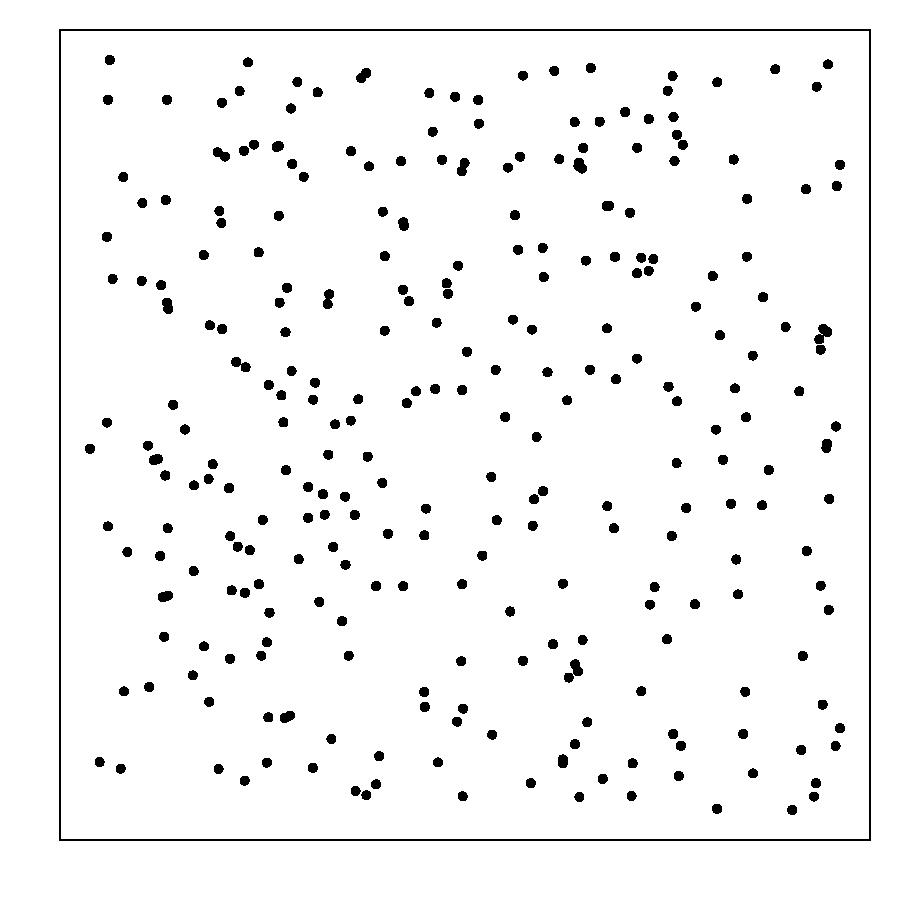
\includegraphics[height=2cm]{Scatterplots4.pdf}
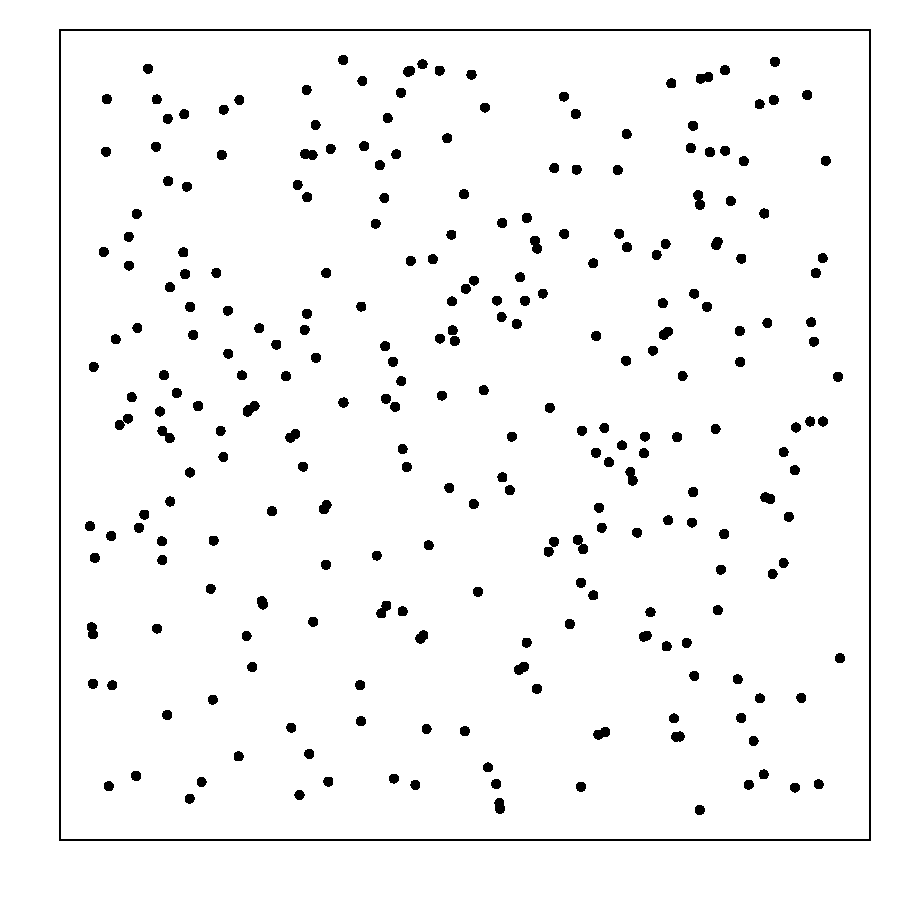
\includegraphics[height=2cm]{Scatterplots5.pdf}
\end{frame}

\begin{frame}{Triangles}
	Which one of the following triangles do you think has the greatest area?

\vspace{0.5cm}
	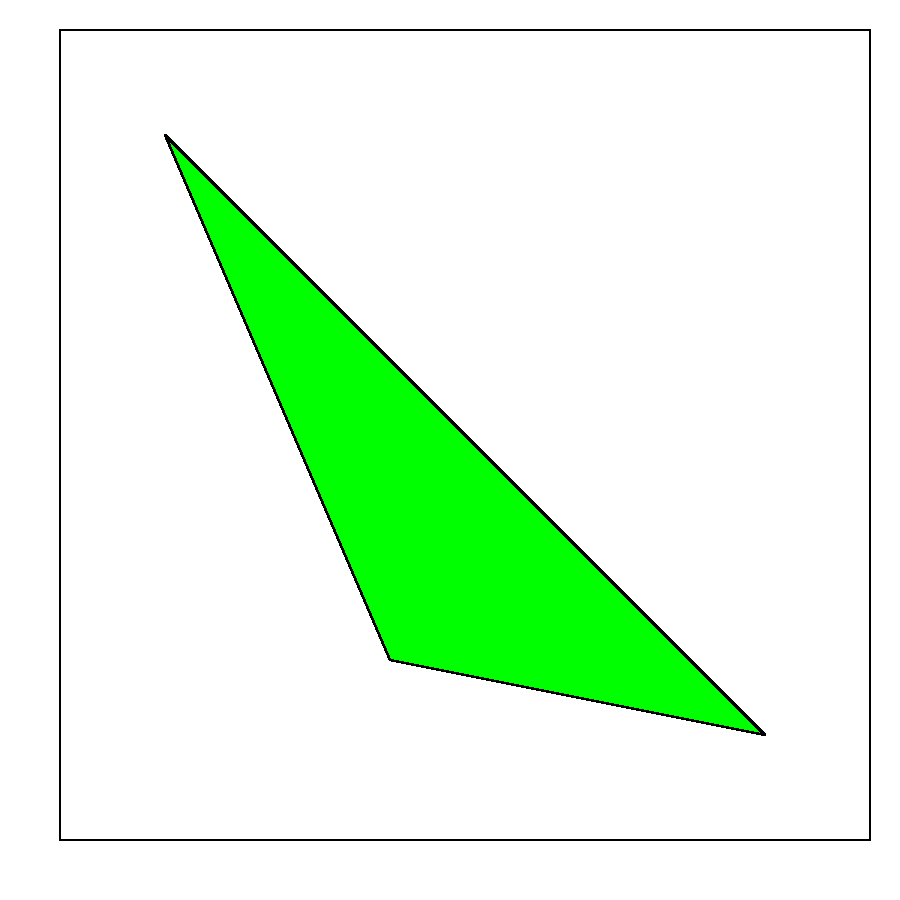
\includegraphics[height=2cm]{Triangles1.pdf}
	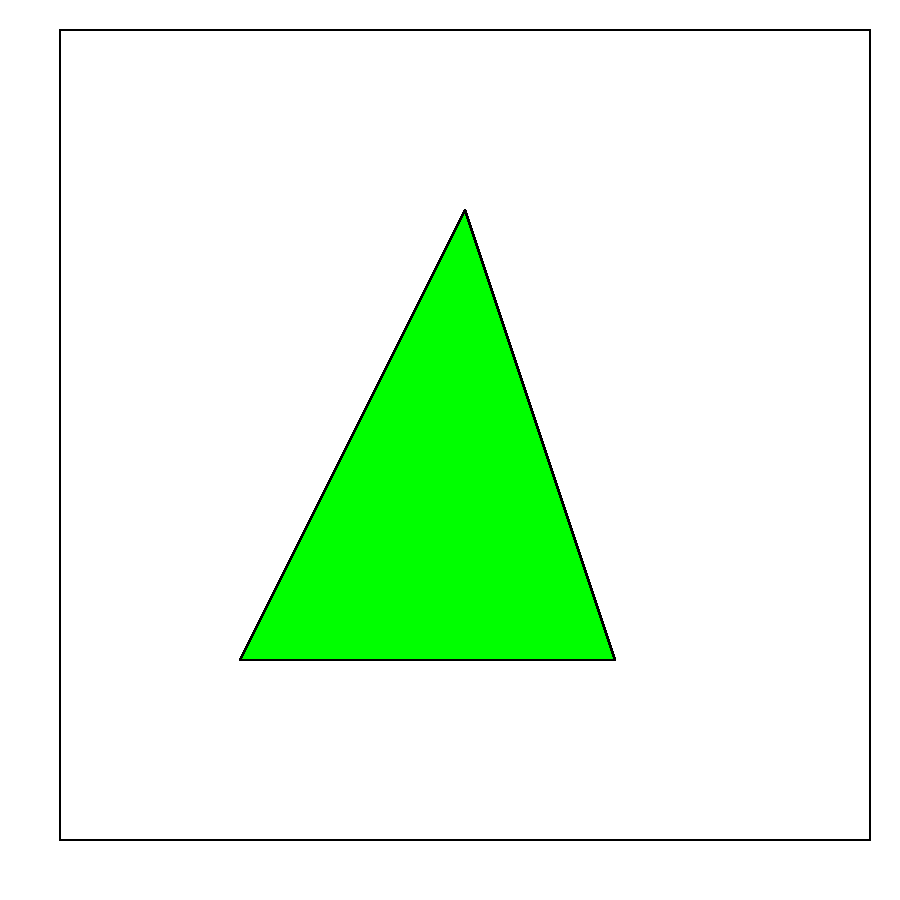
\includegraphics[height=2cm]{Triangles2.pdf}
	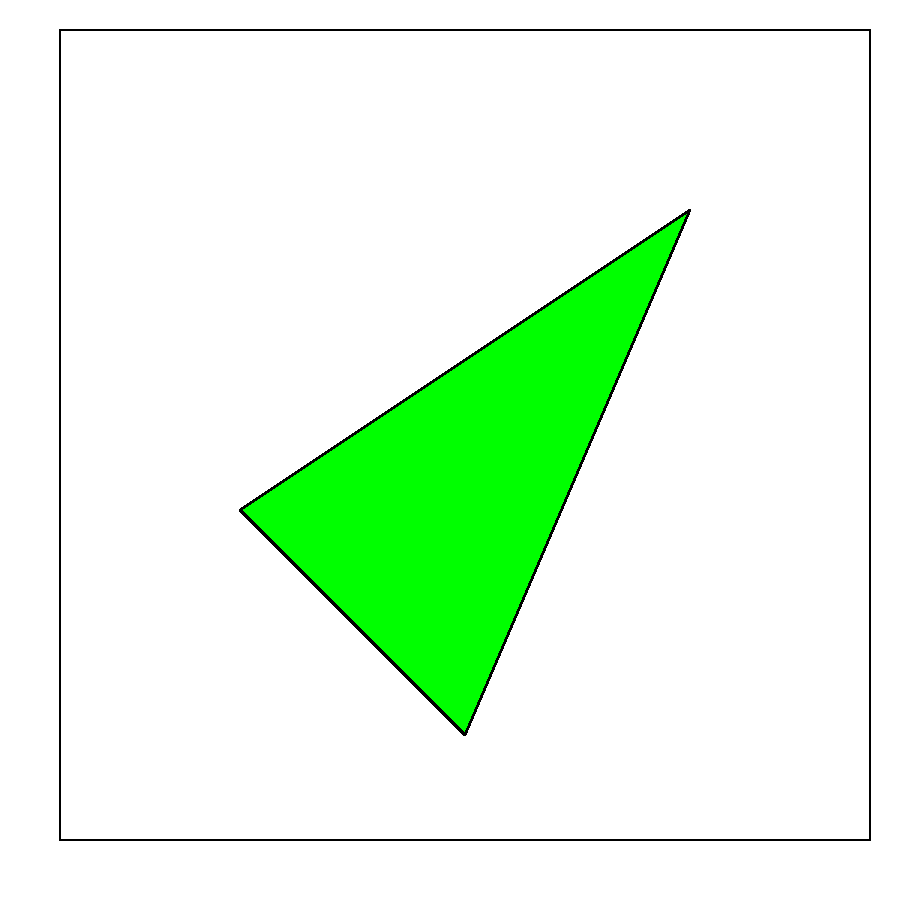
\includegraphics[height=2cm]{Triangles3.pdf}
	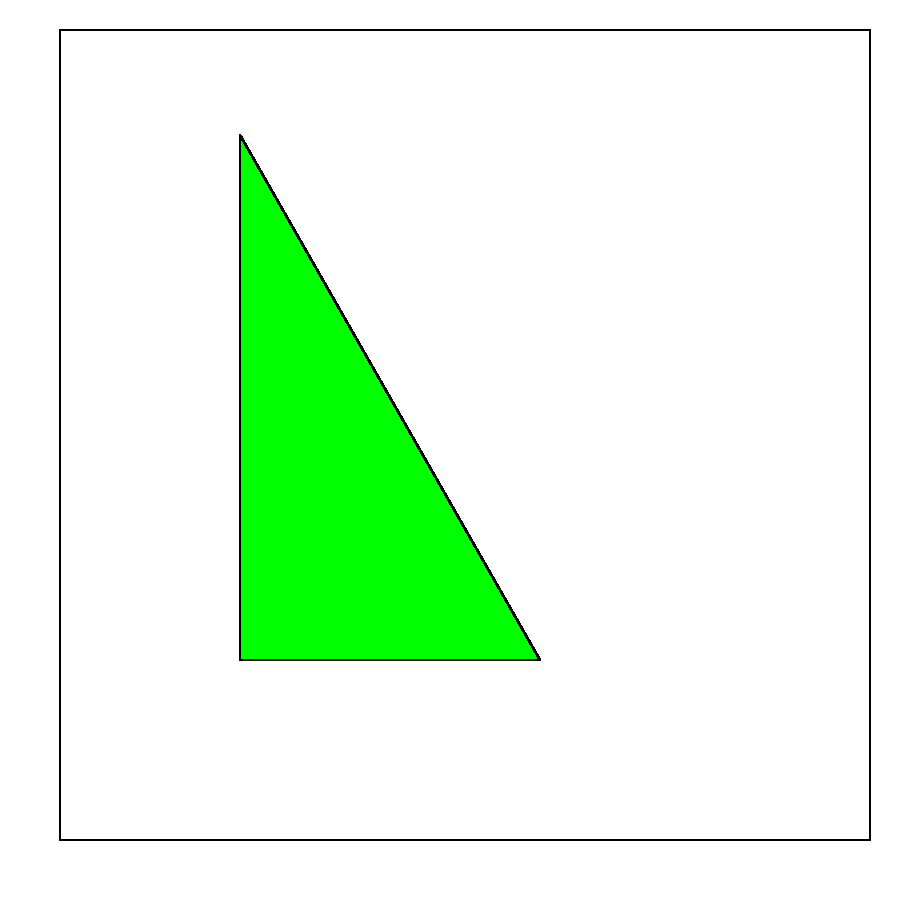
\includegraphics[height=2cm]{Triangles4.pdf}
	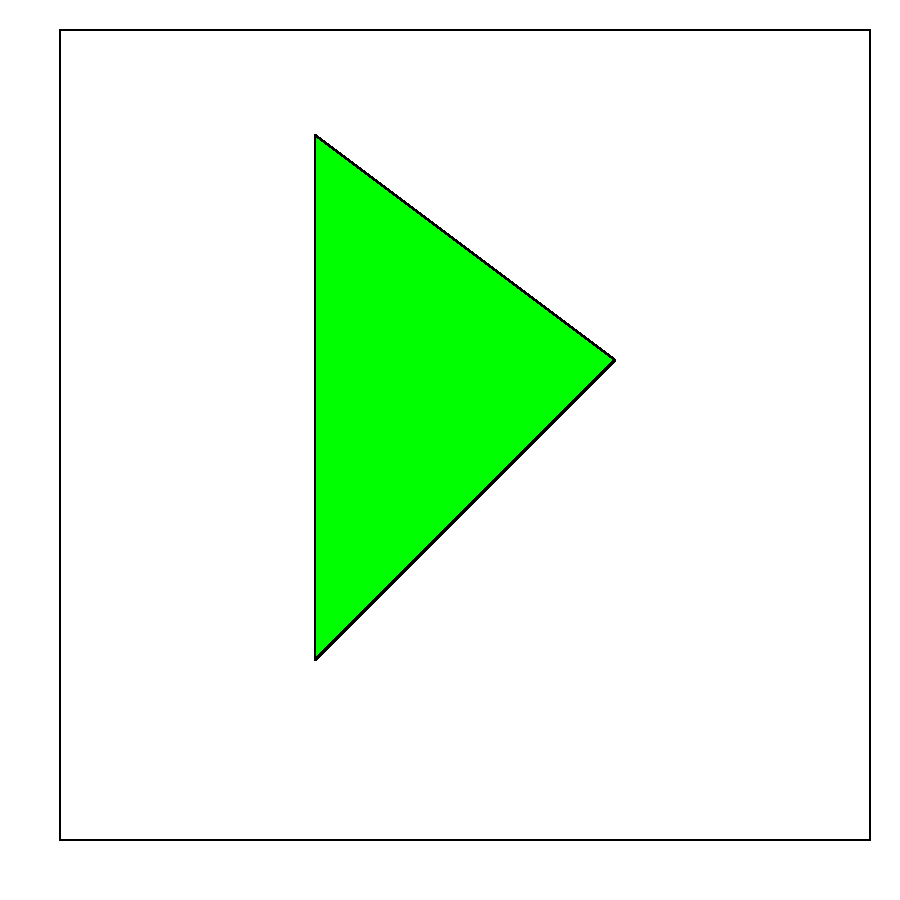
\includegraphics[height=2cm]{Triangles5.pdf}	
\end{frame}

\begin{frame}{Population}
Which one of the following countries do you think has the largest population?

\begin{itemize}
	\item Indonesia
	\item Brazil
	\item Pakistan
	\item Nigeria
	\item Bangladesh
\end{itemize}
\end{frame}

\begin{frame}{Surface area}
Which one of the following countries do you think has the greatest surface area, including inland bodies of water?
	
\begin{itemize}
	\item Canada
	\item United States of America
	\item China
	\item Brazil
	\item Australia
\end{itemize}
\end{frame}

\begin{frame}{Beer}
Below you will find three brands of beer.
You know only the price per sixpack and the average quality ratings made by subjects in a blind taste test.
Given that you had to choose one brand to buy on this information alone, which one would you choose?

\vspace{0.5cm}
\begin{tabular}{cc}
\hline
Price/sixpack & Average quality rating (100 = Best; 0 = Worst) \\ 
\hline
\$9.00 & 50 \\ 
\$13.00 & 70 \\ 
\$15.00 & 70 \\ 
\$14.00 & 75 \\ 
\$15.00 & 80 \\ \hline
\end{tabular}
\end{frame}

\begin{frame}{Cars}
Which one of the following cars would you choose to drive, all other features
begin equal? Ride quality is a on a scale of 0 to 100.

\vspace{0.5cm}
\begin{center}
\begin{tabular}{cc}
\hline
Ride quality & Miles per gallon \\ \hline
60 & 30 \\ 
80 & 24 \\ 
70 & 27 \\ 
55 & 28 \\ 
75 & 22 \\ \hline
\end{tabular}
\end{center}
\end{frame}

\begin{frame}{Restaurants}
Which one of the following restaurants would you choose for your next restaurant meal, based on transportation time (in minutes) and average customer ratings (from
1 to 5).

\vspace{0.5cm}
\begin{center}
\begin{tabular}{cc}
\hline
Transportation time & Rating \\ \hline
34 & 4.4 \\ 
22 & 4.0 \\ 
19 & 3.9 \\ 
7 & 3.5 \\ 
22 & 3.9 \\ \hline
\end{tabular}
\end{center}
\end{frame}

\begin{frame}{Flights I}
Which one of the following flight itineraries would you choose?
All involve two flights, with one layover between them.

\vspace{0.5cm}
\begin{center}
\begin{tabular}{ccc}
\hline
Total inflight time & Layover time & Total itinerary time \\ \hline
4:00 & 1:00 & 5:00 \\ 
3:24 & 1:48 & 5:12 \\ 
3:15 & 2:00 & 5:15 \\ 
3:06 & 2:12 & 5:18 \\ 
2:30 & 3:00 & 5:30 \\ \hline
\end{tabular}
\end{center}
\end{frame}

\begin{frame}{Delayed Choice}
Which one of the following would you choose?

\begin{itemize}
	\item \$200 credited to your bank account immediately.
	\item \$245 credited to your bank account in six months.
	\item \$255 credited to your bank account in one year.
	\item \$315 credited to your bank account in two years.
	\item \$465 credited to your bank account in four years.
\end{itemize}
\end{frame}

\begin{frame}{Phone plans}
Of the following cell phone plans, which one would you choose? In all cases, unlimited calling, text picture and video messages to Canadian and international mobile numbers are included. Excess data usage is billed at \$10 per 500 MB.

\begin{itemize}
	\item 1 GB data per month, \$35 per month.
	\item 2 GB data per month, \$45 per month.
	\item 4 GB data per month, \$49 per month.
	\item 6 GB data per month, \$54 per month.
	\item 8 GB data per month, \$58 per month.
\end{itemize}
\end{frame}

\begin{frame}{Hotel rooms}
Suppose you are staying over two nights in New York city.
Which one of the following hotels would you choose, based on customer ratings and price per night?	

\begin{itemize}
	\item 3.6/5 Scatterplots, \$215 per night
	\item 3.9/5 Scatterplots, \$263 per night
	\item 4.2/5 Scatterplots, \$311 per night
	\item 4.5/5 Scatterplots, \$358 per night
	\item 4.8/5 Scatterplots, \$406 per night
\end{itemize}
\end{frame}

\begin{frame}{Flights II}
Which one of the following flight itineraries would you choose? All involve two
flights and have a total duration of six hours.

\vspace{0.5cm}
\begin{center}
\begin{tabular}{ccc}
\hline
	1st flight & Layover & 2nd flight \\ \hline
	1:30 & 1:15 & 3:15 \\ 
	3:15 & 1:15 & 1:30 \\ 
	2:15 & 1:30 & 2:15 \\ 
	1:30 & 1:45 & 2:45 \\ 
	2:45 & 1:45 & 1:30 \\ \hline
\end{tabular}
\end{center}
\end{frame}

\begin{frame}{Televisions}
Which one of the following televisions would you choose to buy if you
were in the market for a television? All are LED televisions. Resolution
refers to number of horizontal lines. Smart indicates internet connectivity.

\vspace{0.5cm}
\begin{center}
\begin{tabular}{ccccccc}
\hline
Brand & Resolution & Smart & Price (\$) & Screen Size (inches) &  \\ \hline
Sharp & 1080 & Yes & 309 & 32 &  \\ 
Insignia & 720 & No & 209 & 32 &  \\ 
Sony & 720 & Yes & 439 & 32 &  \\ 
Samsung & 1080 & Yes & 459 & 40 &  \\ 
Toshiba & 1080 & No & 409 & 43 &  \\
\hline
\end{tabular}
\end{center}
\end{frame}

\begin{frame}{Coffee}
You need to buy 16oz of ground coffee for a brunch with friends.
Which one of the following ground coffees would you choose?

\vspace{0.5cm}
\begin{scriptsize}
\begin{center}
\begin{tabular}{rcl}
\hline
Price & Fair Trade & Name: Description \\
\hline
18.71 & Yes & Ethiopian Yirgacheffe: vibrant and intensely aromatic, fruity \\
9.99 & No & Colombian Supremo: mellow cup, complex aromas and rich flavours \\
13.72 & Yes & Colombian Organic: medium body, fragrant aroma and mild acidity \\
12.35 & No & Tanzania Peaberry: full bodied coffee, chocolatey aroma, wine-like finish \\
13.46 & No & Sumatra Mandheling: exotic, earthy, bright with low acidity \\
\hline
\end{tabular}
\end{center}
\end{scriptsize}
\end{frame}

\begin{frame}{Charity}
Suppose someone was donating a total of 100 dollars to a combination of charities,
on your behalf.
Which one of the following divisions of the 100 dollars would you choose?

\vspace{0.5cm}
\begin{center}
\begin{tabular}{p{25mm}|p{25mm}|p{25mm}|p{25mm}}
\hline
Arthritis Research Canada &
Canadian Cancer Society &
Canadian Coalition for Firearm Rights &
Coalition for Gun Control \\
\hline
90 & 10 & 0 & 0 \\
35 & 60 & 5 & 0 \\
35 & 60 & 0 & 5 \\
10 & 80 & 10 & 0 \\
10 & 80 & 0 & 10 \\
\hline
\end{tabular}
\end{center}
\end{frame}

\end{document}